%%%%%%%%%%%%%%%%%%%%%%%%%%%%%%%%%%%%%%%%%%%%%%%%%%%%%%%%%%%%%
\subsubsection{物理升级：从双光束到 Airy 多光束模型}

问题1 的双光束模型只考虑了表面反射与衬底界面一次反射两束光的干涉。实际上，光在外延层上下界面之间会发生多次往返反射，每次往返后都有一部分透出表面，所有透出束相干叠加。这一物理过程可由 Airy 公式精确描述\cite{ref-s25}。

三层介质（空气/外延层/衬底）的 Airy 合成反射场为：
\begin{equation}
    \frac{E_r}{E_0} = r_{01} + \frac{(1-r_{01}^2)\,r_{12}(\sigma)\,e^{i\Delta(\sigma)}}{1 + r_{01}\,r_{12}(\sigma)\,e^{i\Delta(\sigma)}}
\end{equation}
其中 $\Delta(\sigma) = 4\pi n_1 d\cos\theta_1\cdot\sigma$ 为往返相位。$r_{12}(\sigma)$ 为复数，由衬底 Drude 介电函数经 Fresnel 公式计算：
\begin{equation}
    \varepsilon(\sigma) = \varepsilon_\infty - \frac{\sigma_p^2}{\sigma(\sigma + i\gamma)}
\end{equation}
$\varepsilon_\infty$ 为高频介电常数，$\sigma_p$ 为等离子体波数，$\gamma$ 为阻尼常数。与 v1.0 的关键区别：(1) $r_{12}$ 不再是常数，而是 $\sigma$ 的复函数；(2) 分母中 $1+r_{01}r_{12}e^{i\Delta}$ 项包含了所有高阶往返束的相干叠加。

\textbf{模型连续性：} 当 $q=|r_{10}r_{12}|\to 0$ 时，Airy 式的一阶截断精确退化为 v1.0/v1.5 双光束式。数值退化测试证实偏差为 $3.9\times 10^{-16}$（机器精度），三个版本是同一物理的三个精度层级，不是三个独立模型。

\subsubsection{多光束干涉可观测的四必要条件}

多光束干涉能否被观测到，取决于四个条件是否同时满足：

\begin{enumerate}
\item \textbf{结构条件（界面平行）：} 外延层上下界面必须平行，保证各往返束以相同方向出射并相干叠加。SiC 和 Si 外延工艺均满足此条件，反射率谱中条纹规整即为证据。

\item \textbf{相干/可分辨条件：} 条纹周期 $\Delta\sigma_{\text{fringe}}\approx 245$--$450$\,cm$^{-1}$ 远大于仪器分辨 $\sim4$\,cm$^{-1}$，往返光程 OPD $23\sim41\,\mu$m 在扫描窗内——条纹可被分辨。注意：谱域测量的相干条件是"可分辨性"而非光源全带宽相干长度。

\item \textbf{透明条件：} 外延层必须透明（$\kappa_1\approx0$），使光束在层内多次往返而不被吸收。轻掺 SiC 和 Si 外延层均满足。

\item \textbf{幅度条件：} 往返因子 $q=|r_{10}r_{12}|$ 必须足够大，使高阶束有可观测的幅度。冻结阈值取 $q\geq0.1$。两材料的 $q$ 值差异显著：
  \begin{itemize}
    \item SiC：$q\approx0.002$--$0.005$（由实测条纹幅度反演，$\sigma_p\approx700$ 档）——远低于阈值，多光束可忽略；
    \item Si：低波数段衬底金属化（$|r_{12}|\to1$，反射率谷值 0\%），$q\gg0.1$——多光束显著。
  \end{itemize}
\end{enumerate}

\textbf{三重数值验证}（确定性验证，非随机）：(1) 闭式与逐束求和（$N=30$ 束）差异 $9.4\times10^{-16}$——Stokes 关系与级数展开正确；(2) 截断误差阶数为 $O(q)$（数值斜率 1.01--1.09），保留三束后降为 $O(q^2)$（斜率 2.03--2.07）；(3) Airy$-$双光束残差的主 FFT 分量为 $2.02\times$ 基频——倍频签名成立，是 Si 判定证据的物理依据。

\subsubsection{Si 判定：出现多光束干涉（证据三选三）}

对 Si 样品（附件3/4），通过四条证据链一致判定出现显著多光束干涉：

\begin{enumerate}
\item \textbf{残差量级：} 双光束模型拟合残差 std 为 8.94\%（10\degree）和 10.14\%（15\degree），分别达噪声水平（$\sim0.04\%$）的 250 倍和 269 倍；lag-1 自相关 0.997，游程检验 $z=-68.7$——残差远非随机噪声，存在强结构。

\item \textbf{可见度衰减：} 条纹可见度从低波数段的 73.8\% 衰减至高波数段的 3.1\%，首末衰减 24--28 倍。双光束模型预测可见度恒定（由 $|r_{01}r_{12}|$ 决定），该衰减是多光束叠加和 Drude 相位频变的联合签名。

\item \textbf{反演厚度差：} v2.0（Airy+Drude）与双光束模型的反演结果差 0.335/0.331\,$\mu$m（10\degree/15\degree），分别为 51$\sigma$ 和 44$\sigma$——远超任何统计涨落。

\item \textbf{四条件核对：} 全部 PASS。幅度条件——低波数段 Si 衬底呈金属化（$|r_{12}|\to1$），$q$ 远超 0.1 阈值。
\end{enumerate}

\begin{figure}[H]
  \centering
  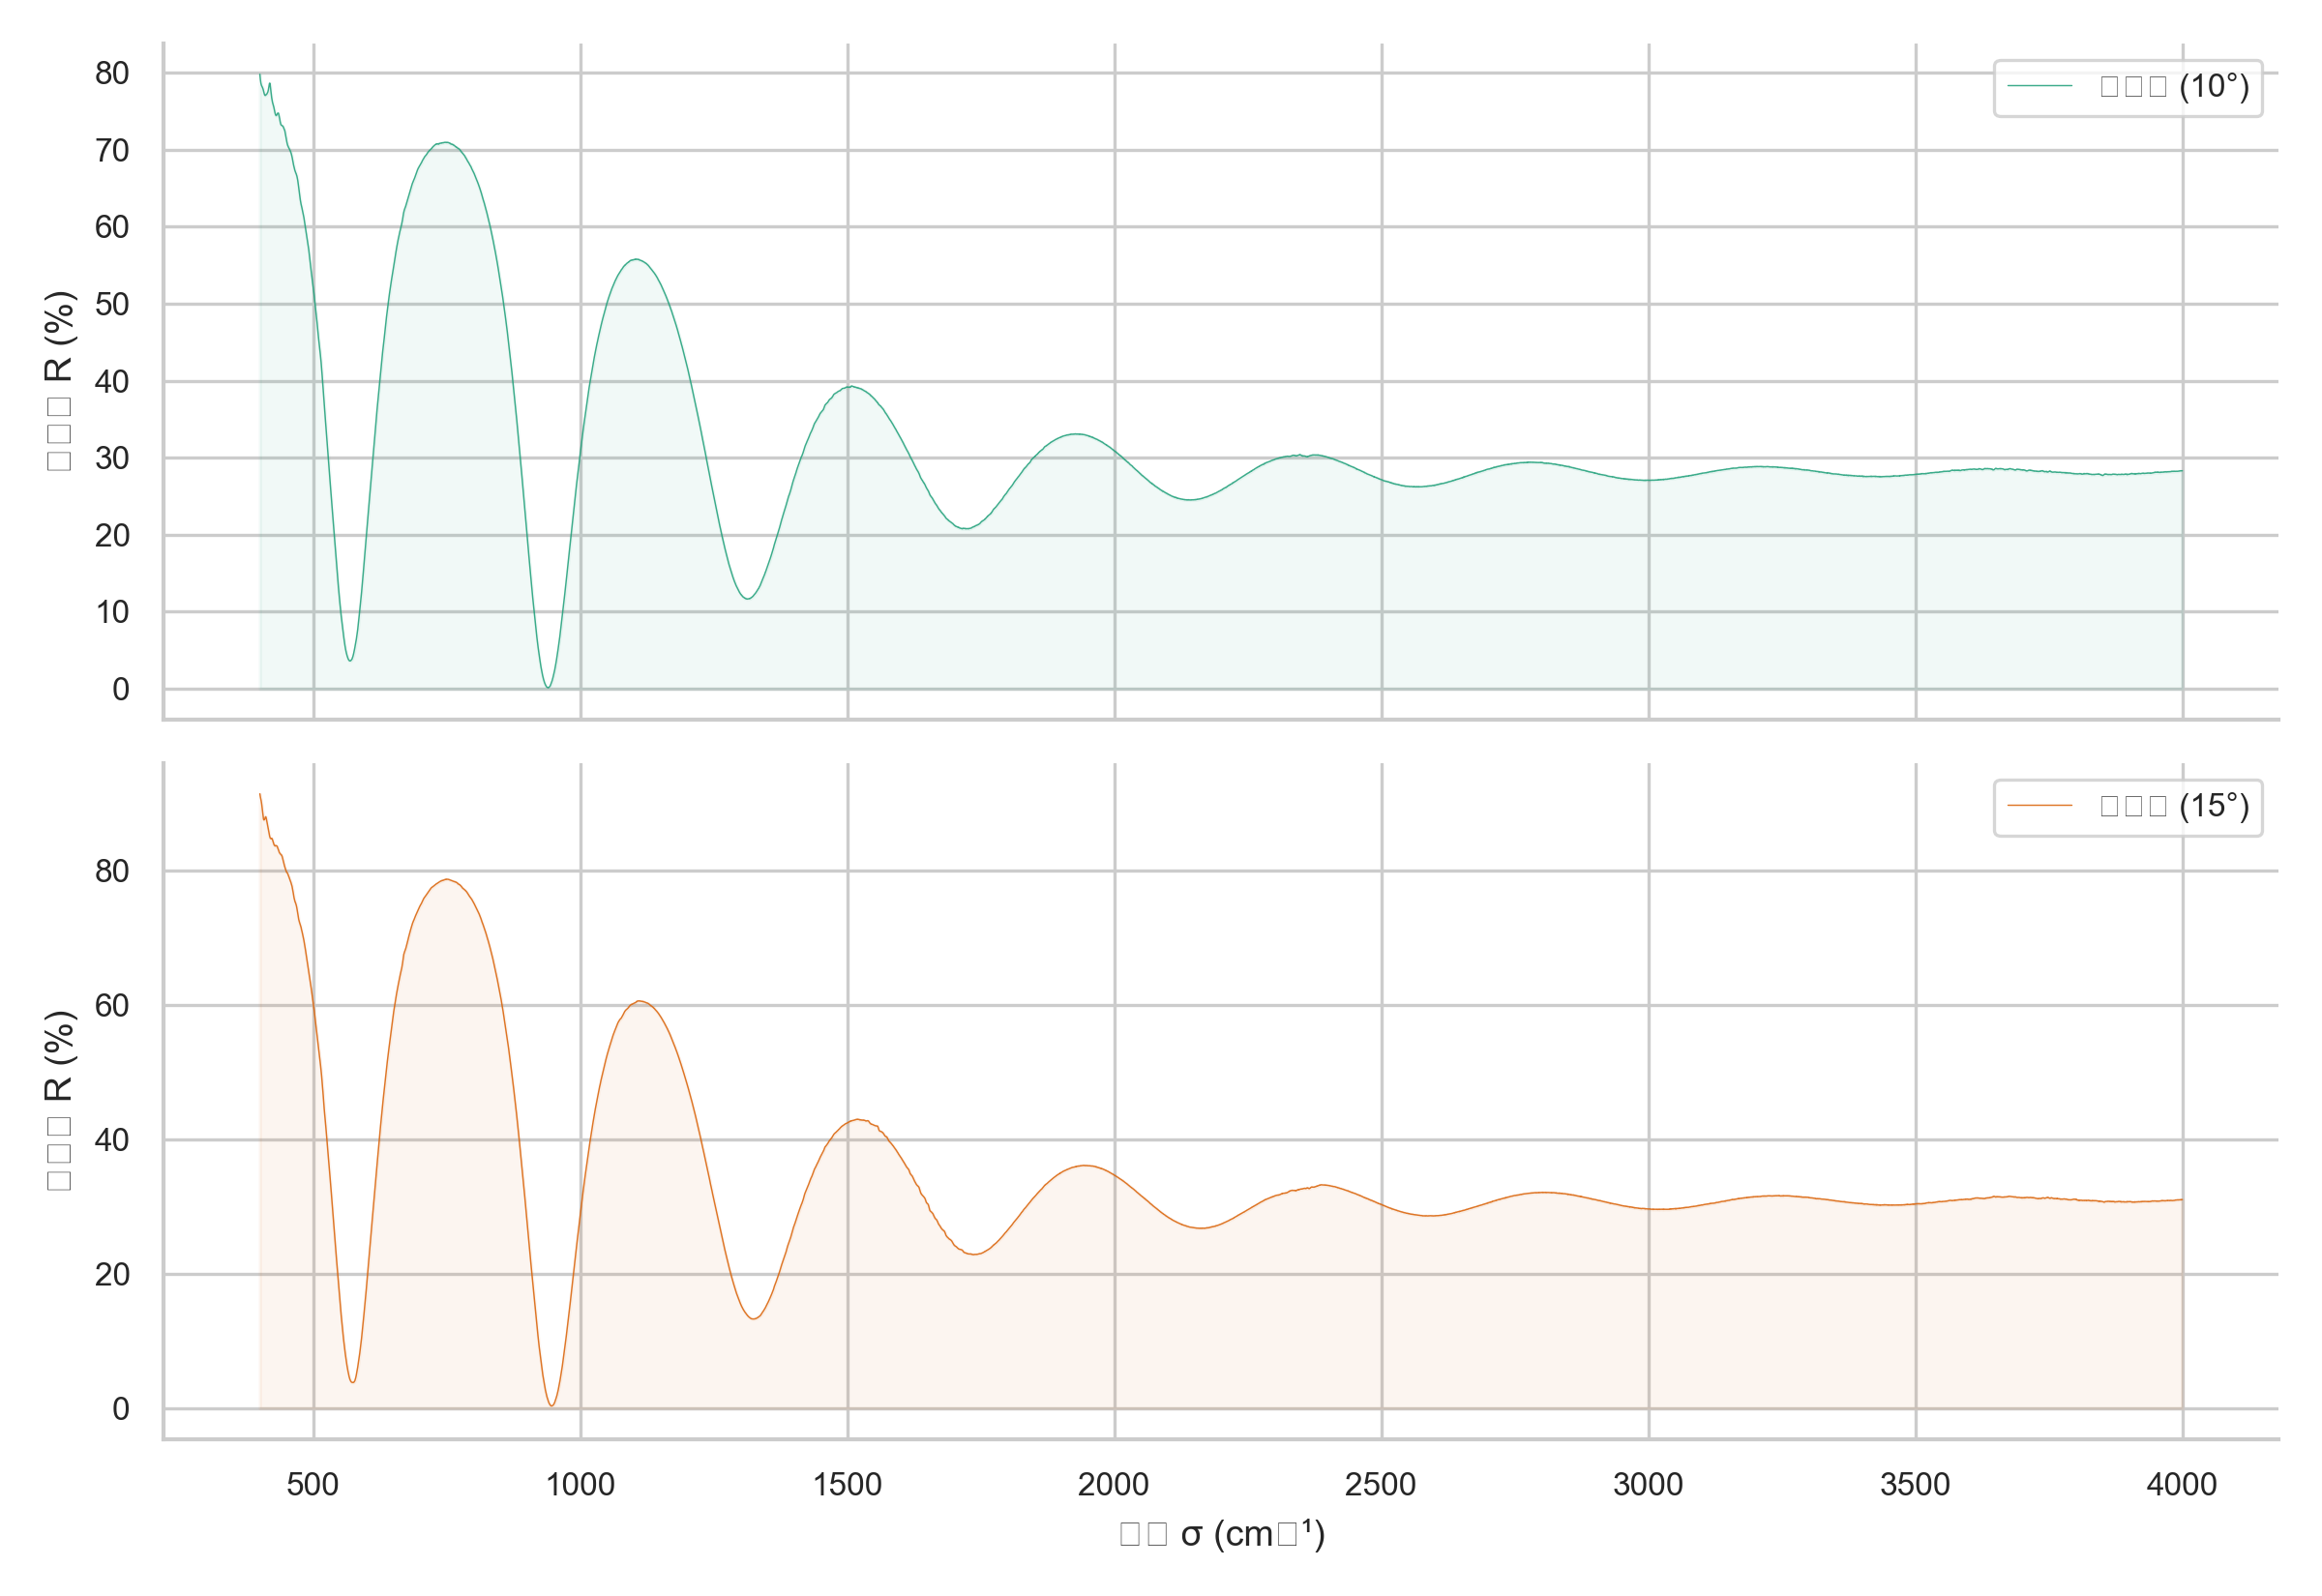
\includegraphics[width=0.92\textwidth]{../../03_结果与图表/最终图表/figB_si_spectrum.png}
  \caption{Si 样品红外反射率谱（附件3/4）}
  \label{fig:si_spectrum}
\end{figure}

\subsubsection{Si 模型与结果}

Si 反演具有特殊性：E1（极值回归）和 E2（谱域 FFT）依赖于条纹周期恒定的假设，而 Si 的条纹周期因 Drude 相位频变而非常数（P1\_Si 分析证实）。因此 Si 反演框架退化为"E3 主 + 双角度互证 + 合成闭环"。

v2.0 E3 以 Airy+固定 Drude 为内核，$\sigma_p$ 选型为 4157\,cm$^{-1}$（扫描内点极小，对应掺杂浓度 $N\approx7.6\times10^{19}$\,cm$^{-3}$，与重掺衬底电阻率口径相容）。合成闭环验证 bias $\leq0.001\,\mu$m。

\textbf{Si 结果：} 外延层厚度 $d = 3.43\,\mu$m，统计不确定度 $\pm0.005\,\mu$m（$d$ 轮廓 $\Delta\chi^2=1$），衬底 $\sigma_p$ 系统区间 $\pm0.15\,\mu$m（扫描跨度 $3.26\sim3.56$）。分角度结果 $3.443/3.419\,\mu$m（差 0.024\,$\mu$m，0.7\%），互证一致。

\subsubsection{SiC 判定与修正（效应分离）}

\textbf{SiC 多光束判定：} 采用 $2\times2$ 效应分离对照（表\ref{tab:effect_separation}），交叉开关 Airy 多光束和固定 Drude 两项升级。

\begin{table}[H]
  \centering
  \caption{SiC 效应分离 $2\times2$ 对照（附件1）}
  \label{tab:effect_separation}
  \begin{tabularx}{\textwidth}{CCCCC}
    \toprule
    模型 & 多光束 & Drude & $\hat{d}$（$\mu$m） & red-$\chi^2$ \\
    \midrule
    M00（v1.5 基准） & 双光束 & 常数 $r_{12}$ & 8.043 & 1862 \\
    M01 & Airy & 常数 $r_{12}$ & 8.055 & 1836 \\
    M10 & 双光束 & 固定 Drude & 9.107 & 1432（$-23\%$）\\
    M11 & Airy & 固定 Drude & 9.107 & 1436 \\
    \bottomrule
  \end{tabularx}
\end{table}

结论：(1) 开启 Airy（M00$\to$M01）red-$\chi^2$ 仅降 1.4\%——\textbf{多光束可忽略}（$q\approx0.002$--$0.005$ 的定量反映）；(2) 开启固定 Drude（M00$\to$M10）red-$\chi^2$ 降 23\%、RMSE 降 12\%——\textbf{衬底 Drude 相位频变是残差主因}。

\begin{figure}[H]
  \centering
  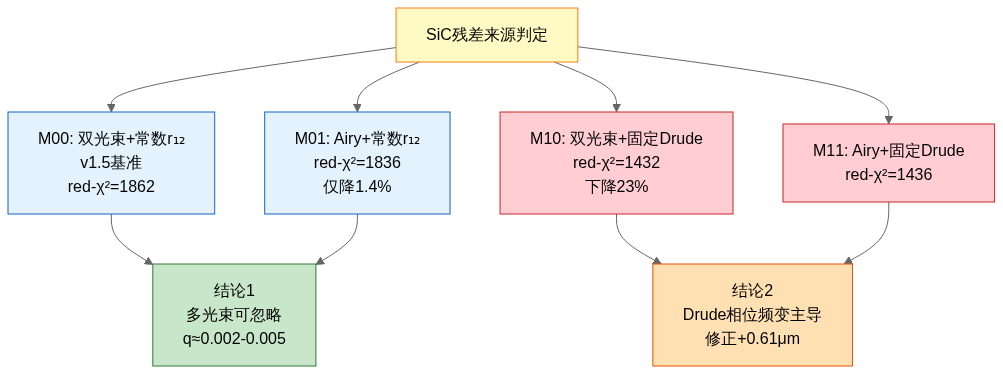
\includegraphics[width=0.90\textwidth]{../../03_结果与图表/最终图表/figM4_effect_separation.png}
  \caption{SiC 效应分离 $2\times2$ 对照（多光束 vs Drude 相位频变）}
  \label{fig:effect_separation_mermaid}
\end{figure}

\textbf{SiC 修正值：} 在 $\sigma_p=4600$\,cm$^{-1}$ 档（跨角度一致性最优，双角度 $|\Delta|$ 从 0.63 缩至 0.064\,$\mu$m，10 倍改善），v2.0 给出 10\degree 8.665 / 15\degree 8.601\,$\mu$m，修正量 $+0.61\,\mu$m（$8.03\to8.64\,\mu$m）。该修正值落在 v1.5 系统区间 $[8.0,8.9]\,\mu$m 的上缘——问题2 的结论无需撤回，但其系统误差主项已被定量化为衬底 Drude 相位频变。$\sigma_p$ 的双口径张力（幅度反演 700 vs 跨角度一致 4600）如实入档，对应 SiC 厚度全区间 $[8.03,9.15]\,\mu$m。

\subsubsection{精度影响量化}

合成数据对照实验（EXP-8）量化了双光束模型在 SiC 形态下的系统偏差（表\ref{tab:bias_exp8}）。v2.0 模型在全工况无偏（$|\text{bias}|\leq0.005\,\mu$m）。

\begin{table}[H]
  \centering
  \caption{双光束模型系统偏差（SiC 形态，15 次实现均值）}
  \label{tab:bias_exp8}
  \begin{tabularx}{\textwidth}{CCCC}
    \toprule
    $\sigma_p$（cm$^{-1}$） & $\bar{q}$ & $d_0=5\,\mu$m 偏差 & $d_0=8\,\mu$m 偏差 \\
    \midrule
    700 & 0.0016 & $+0.033$ & $+1.378$ \\
    1500 & 0.0089 & $+0.023$ & $+1.350$ \\
    4000 & 0.1006 & $+1.378$ & $+1.134$ \\
    \midrule
    v2.0 全工况 & — & \multicolumn{2}{c}{$\leq0.005$} \\
    \bottomrule
  \end{tabularx}
\end{table}

关键发现：(1) 双光束偏差为正（高估），随条纹数增长；(2) 偏差主因是 Drude 相位 chirp 的累积而非多光束幅度（$q$ 最小时偏差依旧大）；(3) 偏差方向以衬底模型区间为条件（Si $+0.33$ 高估 vs SiC 闭环 $-0.14$ 低估），禁止一概而论。